%----------------------------------------------------------------------------
\chapter{Bilineáris filter megvalósítása}
%----------------------------------------------------------------------------

Mivel ez volt az első félév ahol FPGA-val, és a verilog nyelvvel találkoztam, ezért első lépésnek azt tűztem ki célul, hogy megalkossam a bilineáris szűrőt. Ez elég sok trial and error-t tartalmazott, mert nem csak a digitális design, és a Vivado fejlesztői környezet, hanem a verilog nyelv is új volt számomra. 

Elsőnek egy olyan egyszerű modult alkottam meg, amelynek ha megadjuk a kimeneti és bemeneti kép méreteit, akkor képes meghatározni mindegyik kimeneti pixelnek a bemeneti képen a helyzetét. Ezután ezt a helyzetet outputként kiadja a modul, és a testbench visszaadja a 4 környező pixelt. 
Ezek után a 4 egymás melletti pixelből a modul előállítja a bilineáris filterhez szükséges súlyokat, majd végül elvégzi a megfelelő szorzásokat, és kiadja outputnak a kimeneti pixel értékét. 

Később ez a modul bővítve lett, hogy a bemenetre azt is meg lehessen adni, hogy hány csatornán érkeznek be a pixelek. Ha ez az érték 1, akkor szürkeárnyalatos képről beszélünk, és ha ez az érték 3, akkor színes, RGB képről beszélünk.
Ezen kívül egy állapotgépbe rendeztem a modult, hogy a későbbi fejezetben bemutatott sorbufferrel szinkronban tudjon működni a bilineáris filter.

\subsection{Számláló modul}

A Eddig sokat beszéltünk a backwards mappingról és különböző filter algoritmusokról, de arról nem, hogy hogyan is határozzuk meg a kimeneti kép pixeleit a bemeneti képen. Ezt a következő módon valósítottam meg. Raszter iránynak megfelelően, balról jobbra és fentről lefele, egyesével végigmentem a kimeneti kép pixelein. Ez egyszerűen megvalósítható, csak 2 számlálót kell inkrementálni, hogyha az x irányú számláló eléri a sornak a végét, akkor azt reseteljük, és inkrementáljuk az y irányú pixel számlálót. Ha az is eléri az kimeneti kép Y nagyságát, akkor készen vagyunk a képpel, ezeket resetelhetjük. 
Ezzel szinkronban, 2 másik számlálót is működtetünk, amely a mebemeti képen levő helyzetét számolja a kimeneti pixeleknek. Mindig amikor x irányban inkrementáljuk a kimeneti pixel számlálót, akkor az x irányú bemeneti pixel számlálót is inkrementáljuk a kimeneti és bemeneti képek arányaival. Mivel a pixelek számlálását 0 tól kezdjük, ezért ez az arányszám a következő lesz:

\begin{equation}
	scaleX=\frac{outputX-1}{inputX-1}, \quad és \quad scaleY=\frac{outputY-1}{inputY-1}
\end{equation}

Tehát a bemeneti és kimeneti képek méretének arányszáma az az érték, amivel inkrementálni kell a bemeneti kép pixel számlálóját. Ezt a működést a \ref{pic:bilinear_abra} ábra szemlélteti.

\begin{figure}[!ht]
	\centering
	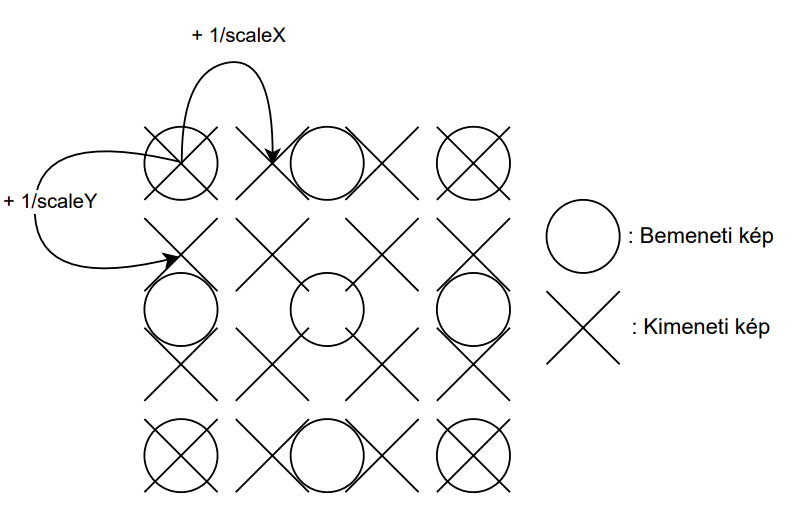
\includegraphics[width=100mm, keepaspectratio]{figures/bilinear_abra.png}
	\caption{A bilineáris filter számlálóinak működése} 
	\label{pic:bilinear_abra}
\end{figure}
\newpage
 Itt viszont észrevesszük, hogy ez az arány szám nem mindig egész szám. Éppen ezért ezt az arányszámot, és a bemeneti pixel számlálót is fix-pontos számként kell ábrázolnunk. Itt meg kellett ismerkednem a fix pontos számábrázolással, ami alapján sikerült is ezt a számláló egységet megvalósítanom. A számábrázolás során fontos volt, hogy a fix pontos számok maximum 18 biten legyenek ábrázolva, hiszen általában egy FPGA-ban ekkora bites számok szorzására képesek a LUT szorzók.

Fontos megjegyezni, hogy ezeket az arányszámokat inputként kell megadni, amelyeknek a legenerálására létrehoztam egy egyszerű python scriptet, melynek ha megadjuk a kimeneti kép és bemeneti kép méreteit, akkor az megadja a fix pontos ábrázolását a scale factoroknak.

A számláló egység tehát képes a kimeneti és bemeneti kép pixelein párhuzamosan végiszámolni. Ehhez készítettem egy szimulációt is, amelyen az látható, ahogy egy 512x512-es képet 800x800 ra méretezünk át. Ekkor ha a kimeneti kép közepén vagyunk, akkor a bemeneti kép közepén kell lenni, ami az \ref{pic:bilin_counter} ábrán levő szimuláción jól látszik hogy megtörténik.

\begin{figure}[!ht]
	\centering
	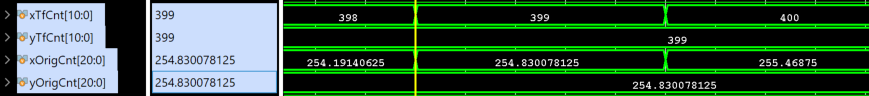
\includegraphics[width=100mm, keepaspectratio]{figures/bilin_counter.png}
	\caption{A bilineáris filter számlálóinak ellenőrzése} 
	\label{pic:bilin_counter}
\end{figure}

Ezután a bemeneti pixel számlálóknak a megfelelő formázása után (egész rész leválasztás) már be lehetett kérni a test bench-től a megfelelő 4 pixel értéket. Miután beérkeztek ezek a pixel értékek, kezdetét vehette a szorzó modul megvalósítása.

\subsection{Szorzó modul}

A szorzó modulban annak megfelelően, hogy hány csatornán érkeznek be a pixelek (1-szürkeárnyalatos, 3-RGB) egy generate blokk segítségével úgy van kiindexelve a bejövő pixel értékekből a megfelelő pixel értékek. Tehát ha 1 csatornáról van szó, akkor a bejövő pixel értékek csak 8 bitesek, de ha 3 csatornás a kép, akkor a bejövő pixelek 24 bitesek. Erre azért van szükség, mert kezdetben csak szürkeárnyalatos képen teszteltem a modult, és később valósítottam meg az RGB képek támogatását is. 

Itt csak megvalósításra kerültek a \ref{eq:mult} egyenletek szorásai. A kihívás itt viszont azt volt, hogy a szorzások megfelelő méretű regiszterekben legyenek tárolva, ne legyen túlcsordulás, ugyanis ha egy pl Q7.0 pixel értéket megszorzunk egy pl Q1.10 méretű együtthatóval, akkor egy Q8.10 méretű számot kapunk, amit csonkítani kell, és még tovább kell szorozni egy másik Q8.0 méretű számmal (felső és alsó interpoláció eredménye), majd végül a függőleges interpolációt is csonkítani kell. 
Ezeken kívül továbbá a megfelelő súlyokat kellő mennyiségő órajellel kellett késleltetni, hogy a felső és alsó interpoláció megfelelő súlyokkal dolgozzon, továbbá egy output data valid jelet is elő kellett állapítani, amit szintén megfelelő mennyiségű órajellel kellett késleltetni a beérkező data input valid jelhez képest.

Ezek után már működött a bilineáris szűrő, de annak érdekében hogy a később megvalósítandó sorbufferekkel szinkronban tudjon működni, egy állapotgépbe rendeztem a rendszer működését.

\subsection{Állapotgép}

A modulnak egy egyszerű állapotgépe van, mely a \ref{pic:bilin_state} ábrán látható.

\begin{figure}[!ht]
	\centering
	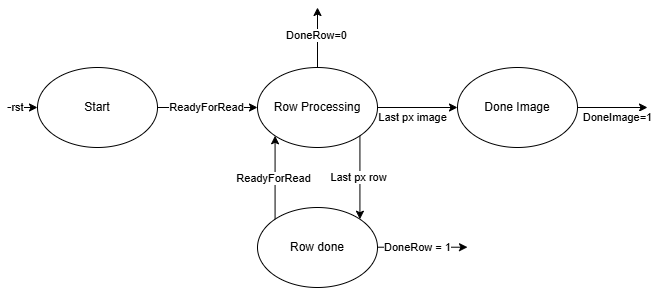
\includegraphics[width=120mm, keepaspectratio]{figures/bilin_state.png}
	\caption{A bilineáris filter állapotgépe} 
	\label{pic:bilin_state}
\end{figure}

A start állapotben inicializálunk minden változót, countert. Ezután, ha legalább 1 órajelig megkapjuk a readyForRead input jelet, akkor az azt jelenti, hogy a sorbuffer beolvasta a megfelelő sorokat, és készen áll az inputok kiadására. Tehát, ha a kimenetre kiírjuk egy pixelnek a koordinátáit (vagyis az oszlopának a sorszámát elég a sorbuffereknél), akkor az 1 órajel múlva meg fog jelenni a bemeneten. 

A processign állapotban egy soron végig halad a filter számlálója, és ezzel párhuzamosan a szorzó egység pár órajel késleltetéssel kiadja a megfelelő kimenő pixel értékét. Ha egy sor végére érünk, akkor a Row done állapotba megyünk át. Ha a kép végére értünk, (sor vége+ oszlopok vége) akkor a done image állapotba térünk.

A Row done állapotban egy soron végigértünk, a doeRow outputot magasra állítjuk, és várjuk hogya readyForRead input magas legyen. Amint ez magasra vált, a doneRow outputot alacsonyra állítjuk, és visszatérünk a Done image állapotba.

Az image Done állapotban a doneimage outputot magasra állítjuk, elkészült a kép. Innen resettel lehet a start állapotba juttatni a modult, és egy újabb kép feldolgozását megkezdeni.

